\chapter{Streuung, Dualität und die Veneziano-Amplitude}

\lectureoverview{Streuung reduziert eine Kollision auf invariante Größen, die sich mit Experimenten vergleichen lassen. Bei vier identischen Teilchen lassen sich diese Größen durch die Mandelstam-Variablen \(s,t,u\) ordnen, von denen nur zwei unabhängig sind. Der gewöhnliche Teilchenaustausch legt dann getrennte direkte und gekreuzte Kanäle nahe. Die Veneziano-Amplitude stellte diese Erwartung auf den Kopf: Eine einzige Funktion enthält Beschreibungen beider Kanäle. In der zweiten Hälfte der Vorlesung wird diese Funktion aus zwei offenen Strings hergeleitet, die sich verbinden, sich als eine einzige oszillierende Kette entwickeln und anschließend wieder aufspalten.}

\section{Was eine Theorie vorhersagen muss}

Fermionische Strings beheben zwei Mängel des rein bosonischen Modells: Sie lassen fermionische Zustände zu und beseitigen nach der geeigneten Projektion das Tachyon. Ihre kritische Raumzeitdimension beträgt zehn statt sechsundzwanzig. Zusätzliche Dimensionen bleiben also bestehen, doch ihre Kompaktifizierung wird zunächst zurückgestellt. Das unmittelbare Thema ist die Streuung.
\editorialnote{Die Aussage, dass das Tachyon fehlt, bezieht sich auf das konsistente Superstring-Spektrum nach der erforderlichen Projektion; das bloße Hinzufügen von Weltflächenfermionen reicht dafür nicht aus.}

Streuung ist nicht notwendigerweise das Interessanteste, was Teilchen tun. Sie ist schlicht der Vorgang, den ein Experiment zuverlässig wiederholen kann. Man schickt festgelegte Teilchen aufeinander zu, registriert die aus der Kollision hervorgehenden Teilchen und erschließt daraus die Dynamik, die im Wechselwirkungsbereich verborgen ist. Eine Theorie wird quantitativ, wenn sie eine komplexe Amplitude liefert
\begin{equation}
  \mathcal A(\hbox{incoming data}\to\hbox{outgoing data}),
\end{equation}
deren Betragsquadrat zusammen mit den üblichen Phasenraumfaktoren die Wahrscheinlichkeit für diesen Ausgang ergibt.

\begin{figure}[H]
  \centering
  
\includegraphics[width=0.72\textwidth]{lecture_06_figure_01.png}
  \caption{Eintreffende Teilchen gelangen in einen Wechselwirkungsbereich als Blackbox, aus dem auslaufende Teilchen hervorgehen; die Zeit ist horizontal dargestellt.}
  \lectureframe{00:02:35}
  \label{fig:l06-black-box}
\end{figure}

Teilchen tragen außerdem Spin, Ladung und Speziesbezeichnungen. Um zunächst die Kinematik herauszuarbeiten, lassen wir vorübergehend alles außer dem Impuls außer Betracht.

\section{Vierimpuls und die Konvention, alle Impulse als einlaufend zu behandeln}

Den Vierimpuls eines Teilchens schreiben wir als
\begin{equation}
  k^\mu=(k^0,\mathbf k)=(E,\mathbf p).
\end{equation}
In der Vorlesung wird die Metrik mit überwiegend positiven Vorzeichen verwendet, also gilt
\begin{equation}
  k^2\equiv \mathbf p^2-E^2.
\end{equation}
Damit lautet die relativistische Dispersionsrelation
\begin{equation}
  E^2-\mathbf p^2=m^2,
  \qquad
  k^2=-m^2.
  \label{eq:l06-mass-shell}
\end{equation}
Eine Änderung des räumlichen Impulses ändert die Energie, doch das Teilchen verlässt dadurch nicht seine Massenschale.

\begin{figure}[H]
  \centering
  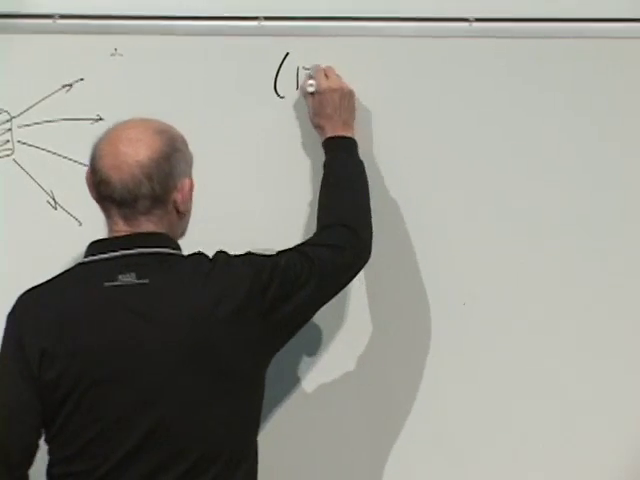
\includegraphics[width=0.66\textwidth]{lecture_06_figure_02.png}
  \caption{Die Massenschalenbedingung in der in der gesamten Vorlesung verwendeten Metrikkonvention.}
  \lectureframe{00:05:56}
  \label{fig:l06-mass-shell}
\end{figure}

Betrachten wir zwei einlaufende Teilchen mit Impulsen \(k_1,k_2\) und zwei auslaufende Teilchen mit physikalischen Impulsen \(q_3,q_4\). Die Energie- und Impulserhaltung ist eine einzige Vierervektorgleichung:
\begin{equation}
  k_1+k_2=q_3+q_4.
  \label{eq:l06-physical-conservation}
\end{equation}
Es ist zweckmäßig, jedem äußeren Bein einen einlaufenden Impuls zuzuordnen:
\begin{equation}
  k_3\equiv-q_3,
  \qquad
  k_4\equiv-q_4.
\end{equation}
Dann gilt
\begin{equation}
  k_1+k_2+k_3+k_4=0,
  \label{eq:l06-all-incoming}
\end{equation}
und für jedes Bein \(k_i^2=-m_i^2\). Nur in dieser Buchhaltungskonvention haben die auslaufenden Teilchen negative Energie; ihre physikalischen Energien bleiben positiv.

\begin{figure}[H]
  \centering
  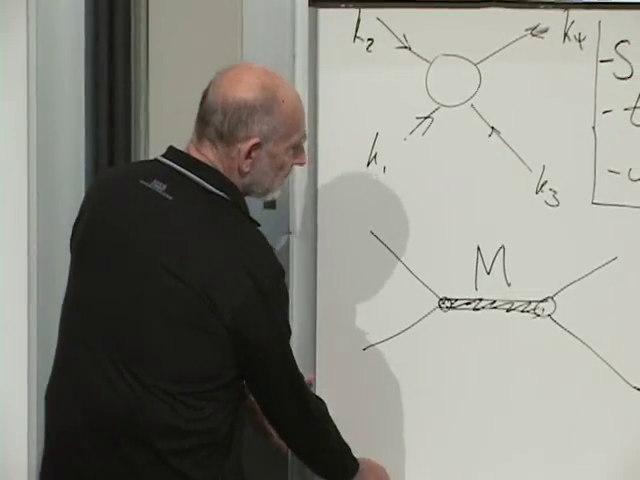
\includegraphics[width=0.68\textwidth]{lecture_06_figure_03.png}
  \caption{Die physikalischen Impulse der auslaufenden Teilchen werden umgekehrt, damit sich alle vier äußeren Impulse symmetrisch als einlaufend behandeln lassen.}
  \lectureframe{00:09:10}
  \label{fig:l06-all-incoming-board}
\end{figure}

Zunächst scheint die Amplitude eine Funktion von sechzehn Komponenten zu sein, \(\mathcal A(k_1,k_2,k_3,k_4)\). Die meisten davon sind redundant. Wir wechseln ins Schwerpunktsystem, richten die einlaufenden Impulse durch eine Drehung entlang einer gewählten Achse aus und nehmen der Einfachheit halber an, dass alle vier Teilchen dieselbe Masse haben. Der einlaufende Zustand ist dann durch eine einzige Größe festgelegt: die Schwerpunktsenergie. Die auslaufenden räumlichen Impulse müssen einander entgegengesetzt sein und denselben Betrag wie das einlaufende Paar haben. Es bleibt nur ihr Ablenkwinkel \(\theta\). Der Prozess hat somit zwei unabhängige kinematische Variablen:
\begin{equation}
  E_{\mathrm{cm}},
  \qquad
  \theta.
  \label{eq:l06-two-data}
\end{equation}

\section{Mandelstam-Variablen}

Die beiden physikalischen Größen in \eqref{eq:l06-two-data} sollten sich ohne Wahl eines Bezugssystems ausdrücken lassen. Mit der Konvention, alle Impulse als einlaufend zu behandeln, definieren wir
\begin{equation}
  \begin{aligned}
    -s&=(k_1+k_2)^2,\\
    -t&=(k_1+k_3)^2,\\
    -u&=(k_1+k_4)^2.
  \end{aligned}
  \label{eq:l06-mandelstam}
\end{equation}
Im Schwerpunktsystem heben sich die räumlichen Anteile von \(k_1+k_2\) auf, daher gilt
\begin{equation}
  s=E_{\mathrm{cm}}^2.
  \label{eq:l06-s-energy}
\end{equation}

Für einen physikalischen auslaufenden Impuls \(q_3=-k_3\) ist
\begin{equation}
  k_1+k_3=k_1-q_3
\end{equation}
der von Bein 1 auf Bein 3 übertragene Impuls. Bei gleichen äußeren Massen und einem Betrag \(p\) des einlaufenden räumlichen Impulses gilt
\begin{equation}
  -t=2p^2(1-\cos\theta),
  \qquad
  -u=2p^2(1+\cos\theta).
  \label{eq:l06-tu-angle}
\end{equation}
Somit enthalten \(t\) und \(u\) die Winkelinformation, die Detektoren messen.

\begin{figure}[H]
  \centering
  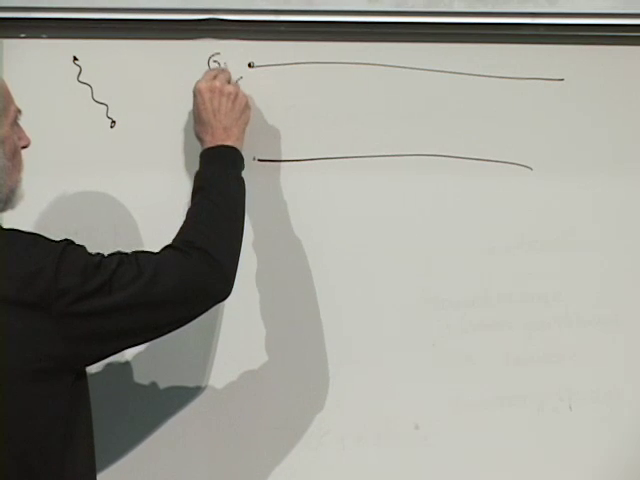
\includegraphics[width=0.74\textwidth]{lecture_06_figure_04.png}
  \caption{Die symmetrischen Definitionen von \(s,t,u\) bei der Konvention, alle Impulse als einlaufend zu behandeln.}
  \lectureframe{00:26:20}
  \label{fig:l06-stu-board}
\end{figure}

Drei Symbole bedeuten nicht, dass drei unabhängige Größen vorliegen. Quadrieren wir \eqref{eq:l06-all-incoming} und verwenden \(k_i^2=-m^2\), erhalten wir bei gleichen Massen
\begin{equation}
  s+t+u=4m^2
  \label{eq:l06-stu-constraint}
\end{equation}
Sobald \(s\) und \(t\) bekannt sind, ist \(u\) festgelegt.

\begin{classroomqa}
\audiencequestion{Kann das Vakuum ein frei bewegtes Teilchen abbremsen, ähnlich wie durch Reibung? \lecturetimestamp{00:27:17}}
\lecturerresponse{Nicht in einem translationsinvarianten Vakuum. Es gibt keinen Ort, an den der fehlende Impuls abgegeben werden könnte; daher verbietet die Impulserhaltung eine solche Reibung. Man kann sich ein Medium oder ein anderes Vakuum vorstellen, das ein bevorzugtes Ruhesystem auszeichnet. Das ist jedoch nicht das hier betrachtete Vakuum.}
\end{classroomqa}

\begin{classroomqa}
\audiencequestion{Warum haben die beiden auslaufenden Teilchen gleiche Energien? \lecturetimestamp{00:27:54}}
\lecturerresponse{Im Schwerpunktsystem müssen ihre räumlichen Impulse gleich groß und entgegengesetzt sein. Beim hier betrachteten Prozess mit gleichen Massen folgt aus gleichen Impulsbeträgen und \(E^2=p^2+m^2\), dass auch die Energien gleich sind. Wären die auslaufenden Massen verschieden, müsste diese letzte Schlussfolgerung angepasst werden.}
\end{classroomqa}

\section{Direkte und gekreuzte Kanäle}

In einem einfachen Diagramm für Punktteilchen bilden die Teilchen 1 und 2 ein Zwischenzustand mit der Masse \(M\), der anschließend in 3 und 4 zerfällt. Bis auf Zählerfaktoren und die Vorschrift für die Pole lautet die charakteristische Abhängigkeit
\begin{equation}
  \mathcal A_s\sim\frac{g^2}{s-M^2}.
  \label{eq:l06-s-channel}
\end{equation}
Dies ist der Prozess im direkten oder \(s\)-Kanal. Dreht man die Verbindung seitwärts, erhält man den Austausch zwischen den beiden äußeren Linien:
\begin{equation}
  \mathcal A_t\sim\frac{g^2}{t-M^2},
  \label{eq:l06-t-channel}
\end{equation}
der Prozess im gekreuzten oder \(t\)-Kanal. Eine dritte Verbindung ergibt
\begin{equation}
  \mathcal A_u\sim\frac{g^2}{u-M^2}.
  \label{eq:l06-u-channel}
\end{equation}

\begin{figure}[H]
  \centering
  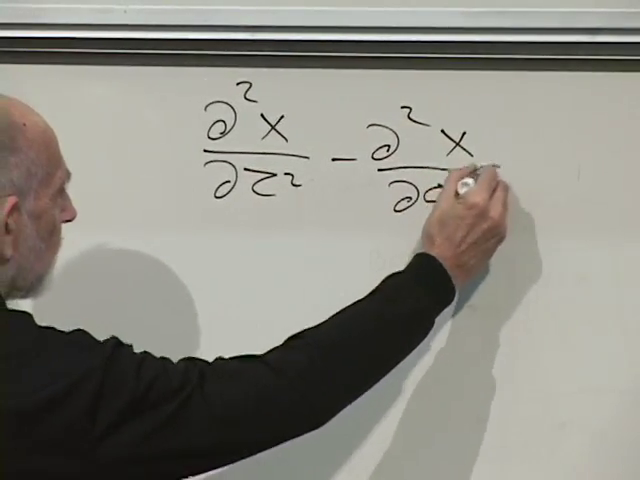
\includegraphics[width=0.72\textwidth]{lecture_06_figure_05.png}
  \caption{Direkte Erzeugung über einen Zwischenzustand und der zugehörige Pol \(g^2/(s-M^2)\); die gekreuzte Verbindung wird auf derselben Tafel aufgebaut.}
  \lectureframe{00:30:50}
  \label{fig:l06-channel-board}
\end{figure}

Der Unterschied ist physikalisch. Auf dieser groben skalaren Ebene hängt \eqref{eq:l06-s-channel} von der Kollisionsenergie, aber nicht vom Winkel ab. Der zusammengesetzte Zustand hat die Einfallsrichtung vergessen, bevor er zerfällt; sein Zerfall ist daher isotrop. Die Austauschamplitude hängt vom Impulsübertrag und damit vom Winkel ab; ein leichtes ausgetauschtes Teilchen begünstigt stark kleine Ablenkungen. Spin würde weitere Winkelabhängigkeiten hinzufügen, doch die Polstruktur ist bereits erkennbar.

\begin{classroomqa}
\audiencequestion{Ergibt der fehlende \(u\)-Kanal einen dritten Term? \lecturetimestamp{00:34:47}}
\lecturerresponse{Ja, sofern die Teilchenidentitäten und Kopplungen diese Verbindung zulassen. Dann nimmt man einen Term mit einem Pol bei \(u=M^2\) auf. Er führt keine neue unabhängige kinematische Variable ein, denn \(s+t+u=4m^2\), ist aber ein eigenständiges Kanaldigramm.}
\end{classroomqa}

\section{Eine Funktion, zwei Kanalbeschreibungen}

Ein einzelner Pol ist ein schlechtes Modell für Mesonenstreuung. Zwei Mesonen können zahlreiche Resonanzen mit einer ganzen Folge von Massen und Drehimpulsen bilden. In den 1960er-Jahren bestand die erste Reaktion darin, weitere Pole im \(s\)-Kanal und im \(t\)-Kanal sowie die erlaubten Pole im \(u\)-Kanal hinzuzufügen. Dann fand man eine wesentlich sparsamere Funktion. In den Einheiten der Vorlesung, in denen die lineare Regge-Trajektorie und ihr Achsenabschnitt in \(s\) und \(t\) aufgenommen sind, lautet sie
\begin{equation}
  \mathcal A_{\mathrm V}(s,t)
  \propto
  \frac{\Gamma(-s)\Gamma(-t)}{\Gamma(-s-t)}.
  \label{eq:l06-veneziano}
\end{equation}
Die Gammafunktion setzt die Fakultät fort:
\begin{equation}
  \Gamma(n)=(n-1)!
\end{equation}
für positive ganze Zahlen.

\begin{figure}[H]
  \centering
  \includegraphics[width=0.68\textwidth]{lecture_06_figure_06.png}
  \caption{Die Veneziano-Amplitude als symmetrischer Quotient von Gammafunktionen.}
  \lectureframe{00:42:25}
  \label{fig:l06-veneziano-board}
\end{figure}

Die Pole von \(\Gamma(-s)\) reproduzieren eine unendliche Folge direkter Kanalresonanzen. Doch derselbe Ausdruck ist unter \(s\leftrightarrow
t\) symmetrisch, sodass seine Pole \(\Gamma(-t)\) eine Entwicklung im gekreuzten Kanal ergeben. Das sind nicht zwei getrennt addierte Beiträge. Eine einzige analytische Funktion lässt beide Beschreibungen zu. Dies ist die ältere Idee der Dualität zwischen direkten Kanalresonanzen und Austauschprozessen im gekreuzten Kanal.

\begin{classroomqa}
\audiencequestion{Wie kann eine Amplitude beide Kanalsummen enthalten, ohne sie zu addieren? \lecturetimestamp{00:43:32}}
\lecturerresponse{Genau das ist die Überraschung. Entwickelt man die Funktion in der Nähe ihrer Pole im \(s\)-Kanal, ordnet sie sich als Folge direkter Resonanzen; entwickelt man sie in der Nähe ihrer Pole im \(t\)-Kanal, ordnet sich dieselbe Funktion als Folge von Austauschprozessen. Um zu erklären, warum beide Lesarten übereinstimmen, braucht es ein mikroskopisches Modell: einen wechselwirkenden String.}
\end{classroomqa}

\section{Ein offener String überstreicht einen Streifen}

Wir parametrisieren einen offenen String durch
\begin{equation}
  0\leq\sigma\leq\pi.
\end{equation}
Die Variable \(\sigma\) bezeichnet keinen Ort in der Raumzeit. Die Einbettung \(X^\mu(\sigma,\tau)\) gibt an, wo sich der so bezeichnete Punkt in der Raumzeit befindet, während \(\tau\) die Entwicklung beschreibt. Ein Punktteilchen überstreicht eine Weltlinie; der bewegte String überstreicht eine zweidimensionale Weltfläche. In der freien Theorie erfüllt jede Einbettungskoordinate die Gleichung
\begin{equation}
  \frac{\partial^2X^\mu}{\partial\tau^2}
  -
  \frac{\partial^2X^\mu}{\partial\sigma^2}
  =0.
  \label{eq:l06-wave-equation}
\end{equation}

\begin{figure}[H]
  \centering
  \includegraphics[width=0.70\textwidth]{lecture_06_figure_07.png}
  \caption{Die Wellengleichung, der jede freie Stringkoordinate auf dem Weltflächenstreifen genügt.}
  \lectureframe{00:49:10}
  \label{fig:l06-wave-equation-board}
\end{figure}

Für die Konstruktion der Streuung ist es hilfreich, den Kontinuumsgrenzfall nicht zu früh zu nehmen. Wir ersetzen jeden String durch \(n\) Massenpunkte, die durch Federn verbunden sind. Die Weltfläche wird zu einer dichten Schar benachbarter Weltlinien, und ihre Normalmoden sind gewöhnliche harmonische Oszillatoren. Zwei einlaufende Ketten können sich an ihren Endpunkten berühren. Bei diesem Ereignis verbindet sie eine neue Feder; sie entwickeln sich während einer Zeit \(\tau\) als eine längere Kette weiter. Später wird eine Feder durchtrennt, sodass zwei auslaufende Ketten entstehen.

\begin{figure}[H]
  \centering
  \includegraphics[width=0.72\textwidth]{lecture_06_figure_08.png}
  \medskip

  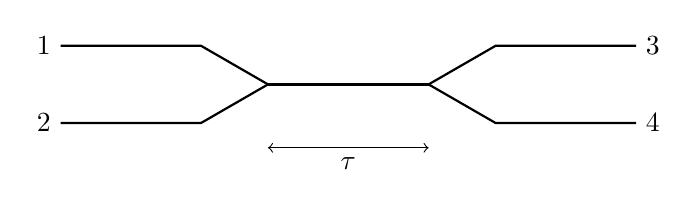
\begin{tikzpicture}[x=0.85cm,y=0.70cm]
    \draw[thick] (0,2.2) -- (2.1,2.2) -- (3.1,1.5);
    \draw[thick] (0,0.8) -- (2.1,0.8) -- (3.1,1.5);
    \draw[thick] (3.1,1.5) -- (5.5,1.5);
    \draw[thick] (5.5,1.5) -- (6.5,2.2) -- (8.6,2.2);
    \draw[thick] (5.5,1.5) -- (6.5,0.8) -- (8.6,0.8);
    \draw[<->] (3.1,0.35) -- node[below] {\(\tau\)} (5.5,0.35);
    \node[left] at (0,2.2) {1};
    \node[left] at (0,0.8) {2};
    \node[right] at (8.6,2.2) {3};
    \node[right] at (8.6,0.8) {4};
  \end{tikzpicture}
  \caption{Zwei diskretisierte offene Strings berühren einander, bilden einen Zwischenstring für die Dauer \(\tau\) und spalten sich wieder auf. Die ursprüngliche Darstellung bewahrt die Konstruktion aus Federn und Weltlinien; das Schema hebt die Verbindungsstruktur hervor.}
  \lectureframe{00:51:25}
  \label{fig:l06-string-joining}
\end{figure}

Die beiden Strings sind nur im Parameterraum nebeneinander gezeichnet. Ihre Positionen in der Raumzeit müssen erst dann benachbart sein, wenn ihre Endpunktkoordinaten tatsächlich zusammenfallen. Die Freiheit der Reparametrisierung erlaubt es, die Ereignisse des Verbindens und Aufspaltens an zweckmäßige Stellen im Diagramm zu setzen; diese geometrische Freiheit wird in der nächsten Vorlesung zur konformen Symmetrie.

\section{Die Oszillatorrechnung Schritt für Schritt}

Die erste Kette habe die Koordinaten \(x_1,\ldots,x_n\), die zweite \(x_{n+1},\ldots,x_{2n}\). Ihre Schwerpunktskoordinaten sind
\begin{equation}
  X_{\mathrm{cm}}^{(1)}
  =\frac1n\sum_{a=1}^{n}x_a,
  \qquad
  X_{\mathrm{cm}}^{(2)}
  =\frac1n\sum_{a=n+1}^{2n}x_a.
  \label{eq:l06-chain-centers}
\end{equation}
Eine Kette mit festem Impuls \(k_1\) hat eine Schwerpunkts-Ebenenwelle, multipliziert mit einem internen Oszillatorgrundzustand:
\begin{align}
  \Psi_1
  &=
  e^{ik_1\cdot X_{\mathrm{cm}}^{(1)}}
  \psi_0(x_1,\ldots,x_n),
  \\
  \Psi_2
  &=
  e^{ik_2\cdot X_{\mathrm{cm}}^{(2)}}
  \psi_0(x_{n+1},\ldots,x_{2n}).
  \label{eq:l06-two-wavefunctions}
\end{align}
Die Faktoren \(\psi_0\) hängen von den Relativkoordinaten ab, nicht von der gemeinsamen Verschiebung der gesamten Kette. Da die einlaufenden Strings zunächst getrennte Quantensysteme sind, gilt
\begin{equation}
  \Psi_{\mathrm{in}}=\Psi_1\Psi_2.
  \label{eq:l06-product-state}
\end{equation}

\begin{figure}[H]
  \centering
  \includegraphics[width=0.76\textwidth]{lecture_06_figure_09.png}
  \caption{Die beiden Impuls-Ebenenwellen und ihre internen Oszillatorgrundzustandsfaktoren, in getrennten Farben dargestellt.}
  \lectureframe{00:58:05}
  \label{fig:l06-wavefunctions-board}
\end{figure}

Beim Verbinden wird der Anteil dieser Wellenfunktion ausgewählt, für den die beiden Endpunktkoordinaten übereinstimmen:
\begin{equation}
  x_n=x_{n+1}.
  \label{eq:l06-endpoint-contact}
\end{equation}
In diesem Augenblick bleiben die übrigen Koordinaten unverändert. Anschließend entwickelt sich der ausgewählte Zustand mit dem Hamiltonoperator \(H_{\mathrm{joined}}\) der einzelnen längeren Kette:
\begin{equation}
  \Psi(\tau)
  =
  e^{-iH_{\mathrm{joined}}\tau}\Psi(0).
  \label{eq:l06-time-evolution}
\end{equation}
Schließlich bildet man sein Skalarprodukt mit einem Produkt auslaufender Stringzustände mit den Impulsen \(q_3,q_4\).

\begin{figure}[H]
  \centering
  \includegraphics[width=0.76\textwidth]{lecture_06_figure_10.png}
  \caption{Die Wellenfunktion der beiden Ketten unmittelbar bevor die Übereinstimmung der Endpunkte erzwungen wird.}
  \lectureframe{00:58:55}
  \label{fig:l06-endpoint-board}
\end{figure}

Die Rechnung ist lang, aber nicht undurchsichtig. Jede interne Koordinate lässt sich in Oszillatormoden zerlegen, sodass das Überlappungsintegral beim Verbinden, die Zeitentwicklung und die abschließende Projektion auf die Gaußsche Oszillatoralgebra zurückgeführt werden. Unbestimmt bleibt nur die Lebensdauer \(\tau\) des verbundenen Strings.

\begin{classroomqa}
\audiencequestion{Werden die schwarzen und roten Wellenfunktionen addiert oder multipliziert? \lecturetimestamp{01:02:26}}
\lecturerresponse{Multipliziert. Der Produktzustand zweier unabhängiger Systeme wird in der Ortsdarstellung durch das Produkt ihrer Wellenfunktionen repräsentiert. Eine Addition würde eine Superposition von Alternativen beschreiben, nicht die gleichzeitige Anwesenheit beider einlaufender Strings.}
\end{classroomqa}

\begin{classroomqa}
\audiencequestion{Warum integrieren wir über die Zwischenzeit \(\tau\)? \lecturetimestamp{01:04:04}}
\lecturerresponse{Dem verbundenen String wird keine feste Lebensdauer zugewiesen. Nach der Regel von Feynman summiert man die Amplituden über alle erlaubten Geschichten. In dieser Beschreibung ist der verbleibende kontinuierliche Parameter einer Geschichte die Zeit zwischen dem Verbinden und dem Aufspalten. Daher wird die Summe zu einem Integral über \(0\leq\tau<\infty\).}
\end{classroomqa}

\section{Von der Ausbreitungszeit zur Betafunktion}

Nach Auswertung der Oszillatorüberlappungen lässt sich das Ergebnis in der Form
\begin{equation}
  \mathcal A(s,t)
  \propto
  \int_0^\infty d\tau\,
  e^{\tau(s+1)}
  \bigl(1-e^{-\tau}\bigr)^{-t-1}
  e^{-\tau}.
  \label{eq:l06-tau-integral}
\end{equation}
Der letzte Faktor \(e^{-\tau}\) bleibt sichtbar, weil er die im nächsten Schritt benötigte Jacobi-Determinante ist. Gleichwertig kann man die erste und die letzte Exponentialfunktion zu \(e^{s\tau}\) zusammenfassen.

\begin{figure}[H]
  \centering
  \includegraphics[width=0.76\textwidth]{lecture_06_figure_11.png}
  \caption{Der Integrand als Funktion der Ausbreitungszeit nach der Oszillatorrechnung; der separate Faktor \(e^{-\tau}\) liefert die Jacobi-Determinante der Variablentransformation.}
  \lectureframe{01:06:45}
  \label{fig:l06-tau-integral-board}
\end{figure}

Nun setzen wir
\begin{equation}
  z=e^{-\tau},
  \qquad
  dz=-e^{-\tau}\,d\tau.
  \label{eq:l06-z-substitution}
\end{equation}
Wenn \(\tau\) von \(0\) bis \(\infty\) läuft, läuft \(z\) von \(1\) bis \(0\). Das Minuszeichen kehrt die Integrationsgrenzen um und ergibt
\begin{equation}
  \mathcal A(s,t)
  \propto
  \int_0^1
  z^{-s-1}(1-z)^{-t-1}\,dz.
  \label{eq:l06-beta-integral}
\end{equation}

\begin{figure}[H]
  \centering
  \includegraphics[width=0.74\textwidth]{lecture_06_figure_12.png}
  \caption{Die Substitution \(z=e^{-\tau}\) macht das Euler-Betaintegral sichtbar.}
  \lectureframe{01:08:49}
  \label{fig:l06-beta-integral-board}
\end{figure}

Dieses Integral ist unmittelbar dort definiert, wo es an den Endpunkten konvergiert, und andernorts durch analytische Fortsetzung. Es ist die Euler-Betafunktion:
\begin{equation}
  B(-s,-t)
  =
  \frac{\Gamma(-s)\Gamma(-t)}{\Gamma(-s-t)}.
  \label{eq:l06-beta-gamma}
\end{equation}

\begin{figure}[H]
  \centering
  \includegraphics[width=0.72\textwidth]{lecture_06_figure_13.png}
  \caption{Die Tafel identifiziert das transformierte Integral mit \(B(-s,-t)\) und beginnt, es wieder in seine Gammafunktionsform zu bringen.}
  \lectureframe{01:12:24}
  \label{fig:l06-beta-gamma-board}
\end{figure}

Die Symmetrie der Kanäle ist nun unmittelbar ersichtlich. Unter \(z\mapsto1-z\) gilt
\begin{equation}
  \int_0^1 z^{-s-1}(1-z)^{-t-1}\,dz
  =
  \int_0^1 z^{-t-1}(1-z)^{-s-1}\,dz.
\end{equation}
Also gilt \(\mathcal A(s,t)=\mathcal A(t,s)\). Ein Prozess, der aus zwei Strings konstruiert wird, die sich verbinden und später wieder aufspalten, enthält automatisch auch die gekreuzte Beschreibung.
\editorialnote{In den Argumenten der Betafunktion lässt die Vorlesung die Regge-Steigung und den Achsenabschnitt unberücksichtigt. In der üblichen Notation ersetzt man \(s,t\) durch die entsprechenden linearen Trajektorien \(\alpha(s),\alpha(t)\). Die Dualität und das Argument der Variablentransformation bleiben unverändert.}

\begin{classroomqa}
\audiencequestion{Erinnert der Quotient der Gammafunktionen an Fakultätsausdrücke aus der Kombinatorik? Gibt es dafür eine unmittelbare physikalische Zählinterpretation? \lecturetimestamp{01:13:22}}
\lecturerresponse{Für ganzzahlige Argumente steht die Betafunktion in Beziehung zu einem Quotienten wie \(n!\,m!/(n+m)!\), doch hier wird kein kombinatorischer Mechanismus behauptet. Dieselbe spezielle Funktion ergibt sich auch aus dem Weltflächenintegral; diese Ähnlichkeit war jedoch nicht der Weg, auf dem die Amplitude gefunden wurde.}
\end{classroomqa}

Der noch verborgene Grund dafür, dass sich dieselbe Weltfläche in beiden Kanälen lesen lässt, ist die konforme Symmetrie. Sie erlaubt es, die Fläche wie Knetmasse zu strecken, ohne die Amplitude zu verändern, und so einen langen Ausbreitungsbereich im direkten Kanal in ein Bild des Austauschs im gekreuzten Kanal zu überführen. Diese geometrische Erklärung wird auf die nächste Vorlesung verschoben.

\section{Was der Streuungstest gezeigt hat}
\enlargethispage{3\baselineskip}
\begingroup
\setlength{\medskipamount}{3pt plus 1pt minus 1pt}

Das diskrete Bild des Verbindens gab Anlass zu einer letzten Reihe von Fragen.

\begin{classroomqa}
\audiencequestion{Wenn sich zwei Ketten aus \(n\) Bestandteilen an ihren Endpunkten verbinden, besteht das Ergebnis dann aus \(2n-1\) Bestandteilen, und könnte sich dadurch die Fermionparität ändern? \lecturetimestamp{01:16:16}}
\lecturerresponse{Im hadronischen Endpunktbild kann man das sich berührende Endpunktpaar als Teilchen-Antiteilchen-Paar auffassen, das annihiliert. Die Anzahl verringert sich also um zwei, nicht um eins. Im Kontinuumsgrenzfall ist der endliche Unterschied zwischen \(2n\) und \(2n-2\) unerheblich, die Erhaltung der Fermionparität dagegen nicht. Die Gitterbestandteile dienen nur als Regulator für den kontinuierlichen String; sie sind keine buchstäblich fundamentalen Kügelchen.}
\end{classroomqa}

\begin{classroomqa}
\audiencequestion{Wird die spätere Diskussion die vollständige Mathematik der Superstrings behandeln? \lecturetimestamp{01:18:05}}
\lecturerresponse{Es werden nur ausgewählte Konsequenzen herangezogen. Der unmittelbare Weg führt über die Symmetrie der Weltfläche und die Kompaktifizierung zu einem anderen Ansatz, der Mitte der 1990er-Jahre entwickelt wurde: der M-Theorie. Damit soll dieselbe Physik aus einer Perspektive erschlossen werden, aus der mehrere ansonsten komplizierte Aspekte transparent werden.}
\end{classroomqa}

\begin{classroomqa}
\audiencequestion{War diese Verknüpfungsregel lediglich ein Hinweis aus Mesonenkollisionen? \lecturetimestamp{01:20:02}}
\lecturerresponse{Die Mesonenstreuung lieferte den historischen Hinweis, doch die Regel gilt allgemein für offene Strings. Dieselbe Topologie beschreibt Kollisionen von Photonen offener Strings und anderen offenen Stringzuständen. Zwei geschlossene Strings vereinigen und trennen sich nach einer analogen Konstruktion, bei der sich im Zwischenbereich ein geschlossener String befindet.}
\end{classroomqa}

\begin{classroomqa}
\audiencequestion{Gilt die Rechnung nur, wenn die Stringzustände Fermionen sind? \lecturetimestamp{01:20:56}}
\lecturerresponse{Nein. Die ursprüngliche Veneziano-Rechnung gehört zur bosonischen Theorie offener Strings. Superstrings erfordern zusätzliche fermionische Freiheitsgrade und verändern Details des Integranden, doch die Logik des Zusammenfügens, der Ausbreitung, der Projektion und der Weltflächen-Dualität bleibt eng analog.}
\end{classroomqa}

Einen Spin-eins- oder Spin-zwei-Zustand im Oszillatorspektrum zu finden, war ein vielversprechender Hinweis, aber kein entscheidender Beleg. Der stärkere Test waren ihre Streuamplituden. Photonamplituden erfüllen die Identitäten, die mit Ladungserhaltung und Eichinvarianz verbunden sind; Gravitonamplituden erfüllen die entsprechenden Bedingungen für ein masseloses Spin-zwei-Feld. Die Stringzustände bestanden diese Tests in Wechselwirkungen mit massiven und masselosen Zuständen sowie untereinander. Deshalb wurden die Bezeichnungen Photon und Graviton zu physikalischen Identifikationen und blieben nicht bloße Vermutungen auf Grundlage der Polarisationszählung.
\editorialnote{In moderner Sprache werden diese Tests durch die Entkopplung unphysikalischer Polarisationen, Eich-Ward-Identitäten und die universelle Niederenergiekopplung des masselosen Spin-zwei-Zustands ausgedrückt.}

\begin{classroomqa}
\audiencequestion{Woher stammt die elektrische Ladung selbst in der Stringbeschreibung? \lecturetimestamp{01:24:03}}
\lecturerresponse{Diese Frage bleibt am Ende der Vorlesung offen. Ihre Beantwortung erfordert die innere Struktur und die Endpunktstruktur der Stringtheorie, die noch nicht eingeführt wurden. Daher gehört sie in die anschließende Diskussion und nicht zu dieser Herleitung der Streuung.}
\end{classroomqa}
\endgroup
